\documentclass{standalone}
\usepackage{tikz}
\usepackage{circuitikz}

\begin{document}
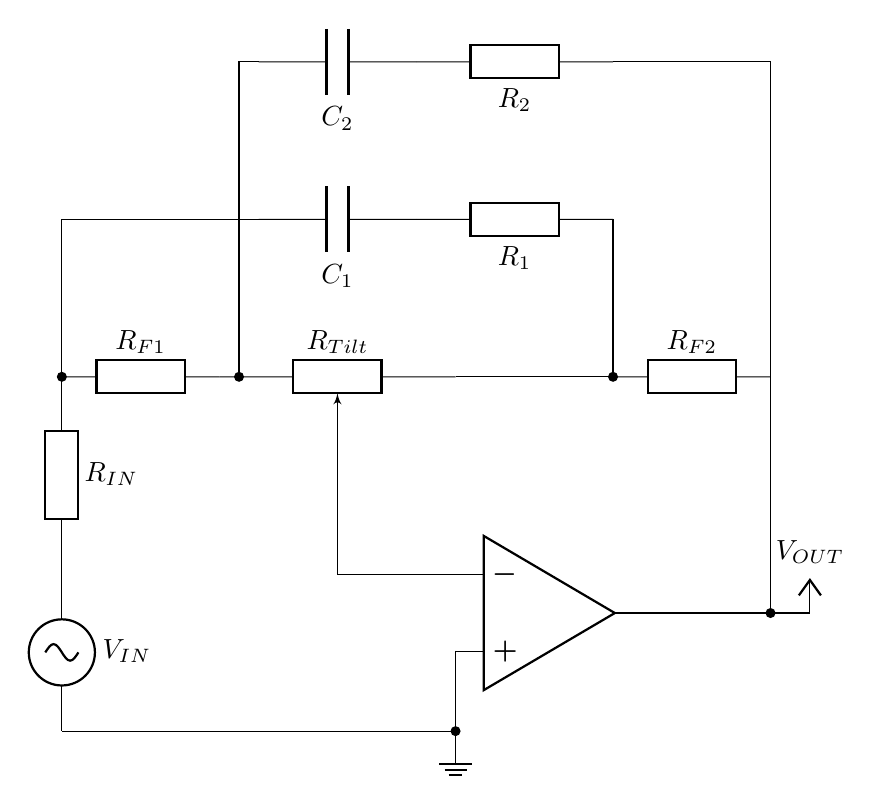
\begin{tikzpicture}
	\draw (2, 6.5) to[sinusoidal voltage source, l=$V_{IN}$] (2, 4.5);

	\draw (2, 9) to[european resistor, l=$R_{IN}$] (2, 6.5);
	\draw (9, 11) to[european resistor, l=$R_1$] (6.5, 11);
	\draw (9, 13) to[european resistor, l=$R_2$] (6.5, 13);
	\draw (4, 9) to[european resistor, l_=$R_{F1}$] (2, 9);
	\draw (11, 9) to[european resistor, l_=$R_{F2}$] (9, 9);

	\draw (7, 9) to[european potentiometer, l_=$R_{Tilt}$] (4, 9);

	\draw (4.5, 11) to[capacitor, l_=$C_1$] (6.5, 11);
	\draw (4.5, 13) to[capacitor, l_=$C_2$] (6.5, 13);

	\node[op amp] at (8.19, 6) {};

	\draw (2, 9) -- (2, 11) -- (4.5, 11);
	\draw (2, 4.5) -- (7, 4.5);
	\draw (4.5, 13) -- (4.25, 13) -- (4.25, 9);
	\draw (7, 6.49) -- (5.5, 6.49) -- (5.5, 8.44);
	\draw (7, 9) -- (9, 9);
	\draw (7, 5.52) -- (7, 4.5);
	\draw (9, 11) -- (9, 9);
	\draw (9, 13) -- (11, 13) -- (11, 9);
	\draw (9.38, 6.01) |- (11.5, 6);
	\draw (11, 9) -- (11, 6);

	\node[ground] at (7, 4.5) {};
	\node[vcc] at (11.5, 6) {$V_{OUT}$};
	\node[circ] at (11, 6) {};
	\node[circ] at (2, 9) {};
	\node[circ] at (4.25, 9) {};
	\node[circ] at (7, 4.5) {};
	\node[circ] at (9, 9) {};

\end{tikzpicture}
\end{document}